\section{Static Load Balancing}
\label{sec:static-load-balancing}

% techinical details
In the original ParSplice implementation, each cache node as much memory as it
wants to store segment coordinates. We limit the size of the cache using an LRU
eviction policy, where the penalty for a cache miss is retrieving the data from
the persistent database.  We evict keys (if necessary) at every operation
instead of when segments complete because the cache fills up too quickly
otherwise and it reduces the overhead of key eviction.

% results: cache size trade-offs
\begin{figure}[t]
  \noindent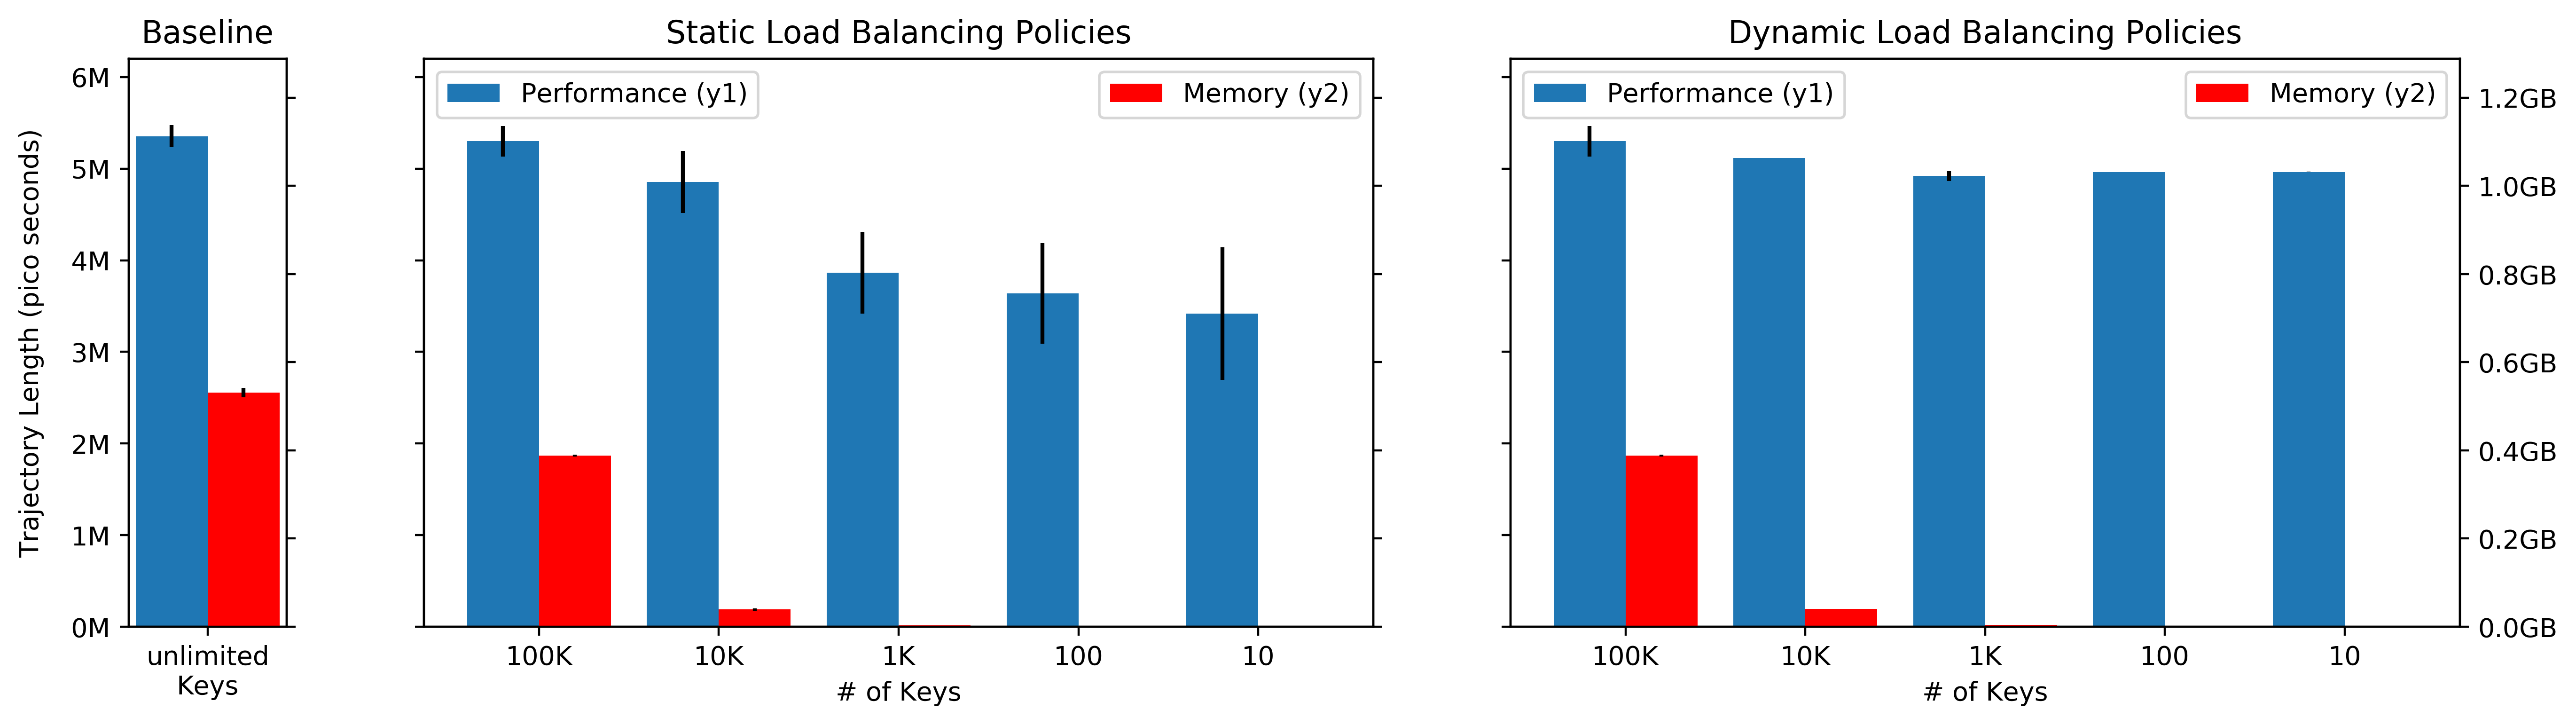
\includegraphics[width=0.4\textwidth]{figures/methodology-tradeoff.png}\\
  \caption{The performance and resource utilzation trade-off for different
  cache sizes, which are enumerated along the \(x\) axis. ``Baseline" is
  ParSplice unmodified and the ``Static  Policies" limit the size of the
  cache to demonstrate the memory savings of smaller keyspaces on cache nodes.
  \label{fig:methodology-tradeoff}}
\end{figure}

The results for different cache sizes for a growth rate of 100K over a 2.5 hour
run is shown in Figure~\ref{fig:methodology-tradeoff}.  ``Baseline" is the
performance of unmodified ParSplice  measured in trajectory duration
(\(y\)-axis) and utilization is measured with memory footprint (\(y2\) axis) of
just the cache.  ``Static Load Balancing Policies" shares the \(y\)-axis and
shows the trade-off for different cache sizes. The error bars are the standard
deviation of 3 runs. 

% results: raw numbers
Although the keyspace grows to 150K, a 100K key cache achieves 99\% of the
peformance. Decreasing the cache degrades performance and predictability.
While this result is not unexpected, it nonetheless achieves our goal of
showing the benefits of load balancing keys across nodes and that smaller
caches on each node are an effective way to save memory without completely
sacrificing performance.
